% begin module e-def
\begin{frame}
\[
\text{If}\quad  f(x) = a^x, \quad \text{then}\quad f'(x) = f'(0)a^x .
\]
The formula above is simplest when $f'(0) = 1$.  Since $\lim\limits_{h\rightarrow 0}\frac{2^h-1}{h}\approx 0.69$ and $\lim\limits_{h\rightarrow 0}\frac{3^h-1}{h}\approx 1.10$, we expect there is a number $a$ between 2 and 3 such that $\lim\limits_{h\rightarrow 0}\frac{a^h-1}{h} = 1$.  
\uncover<2->{
\begin{definition}[$e$]
$e$ is the number such that $\lim\limits_{h\rightarrow 0}\frac{e^h-1}{h} = 1$.
\end{definition}
}

\begin{columns}
\column{.3\textwidth}
\psset{xunit=1.1cm, yunit=1.1cm}
\begin{pspicture}(-1.3, -0.5)(1.4,2.5) 
\psframe*[linecolor=white](-1.3,-0.5)(1.5,2.5) 
\psaxes[labels=none]{<->}(0,0)(-1.3, -0.5)(1.3,2.5)
\psplot[linecolor=red, plotpoints=1000]{-1.3}{1.3}{2 x exp}
\rput[r](-0.2, 1.1){\footnotesize $y=2^x$}
\rput[l](0.2, 0.8){\tiny $m\approx 0.693147$} 
\psline[linecolor=blue](-1.3,0.098908665)(1.3, 1.901091335)
\end{pspicture}
%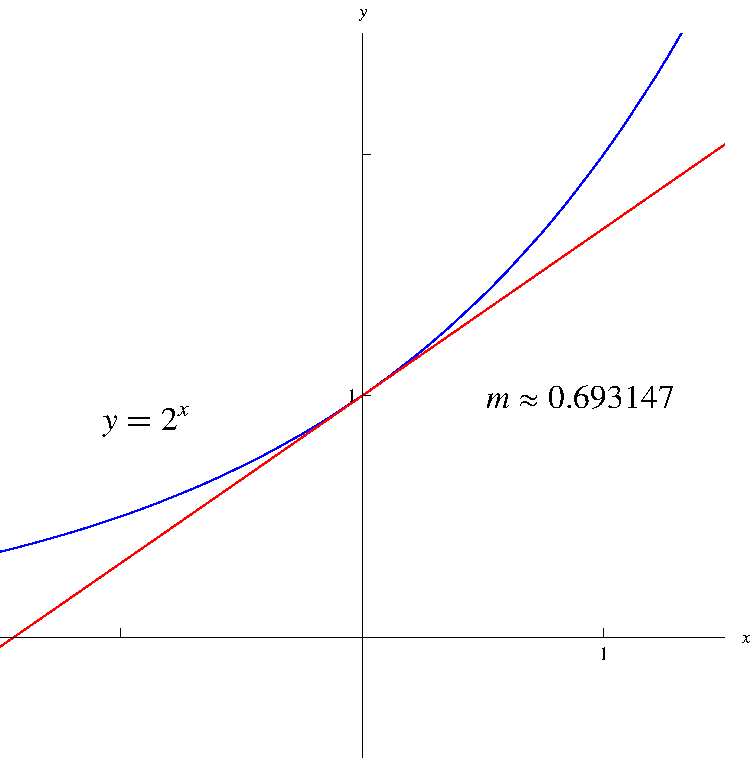
\includegraphics[height=4cm]{exponential-functions/pictures/exp-tangent-two.pdf}%
\column{.3\textwidth}
\uncover<handout: 1|3->{%
\psset{xunit=1.1cm, yunit=1.1cm}
\begin{pspicture}(-1.3, -0.5)(1.4,2.6) 
\psframe*[linecolor=white](-1.3,-0.5)(1.4,2.6) 
\psaxes[labels=none]{<->}(0,0)(-1.3, -0.5)(1.3,2.5)
\psplot[linecolor=red, plotpoints=1000] {-1.3}{0.901091335}{2.718281828 x exp}
\rput[r](-0.2, 1.1){\footnotesize $y=e^x$}
\rput[l](0.2, 0.8){\tiny $m=1$}
\psline[linecolor=blue](-1.3, -0.3)(1.3,2.3) 
\end{pspicture}
%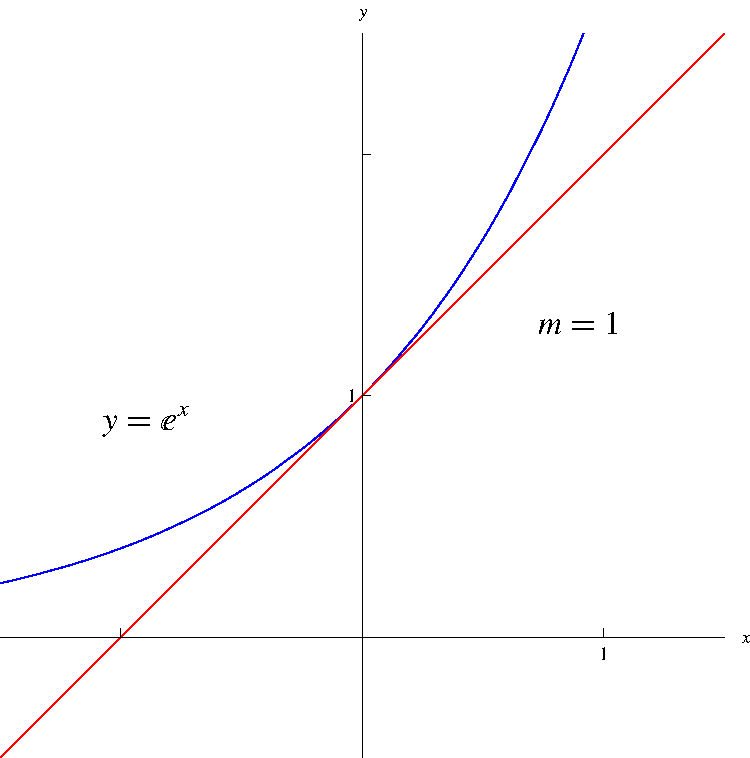
\includegraphics[height=4cm]{exponential-functions/pictures/exp-tangent-e.pdf}%
}%
\column{.3\textwidth}
\psset{xunit=1.1cm, yunit=1.1cm}
\begin{pspicture}(-1.3, -0.5)(1.4,2.6) 
\psframe*[linecolor=white](-1.3,-0.5)(1.4,2.6) 
\psaxes[labels=none]{<->}(0,0)(-1.3, -0.5)(1.3,2.5)
\psplot[linecolor=red, plotpoints=1000]{-1.3}{0.82020868}{3 x exp}
\rput[r](-0.2, 1.1){\footnotesize $y=3^x$}
\rput[l](0.2, 0.8){\tiny $m\approx 1.09861$} 
\psline[linecolor=blue](-1.3, -0.428195975)(1.3,2.428195975)
\end{pspicture}
%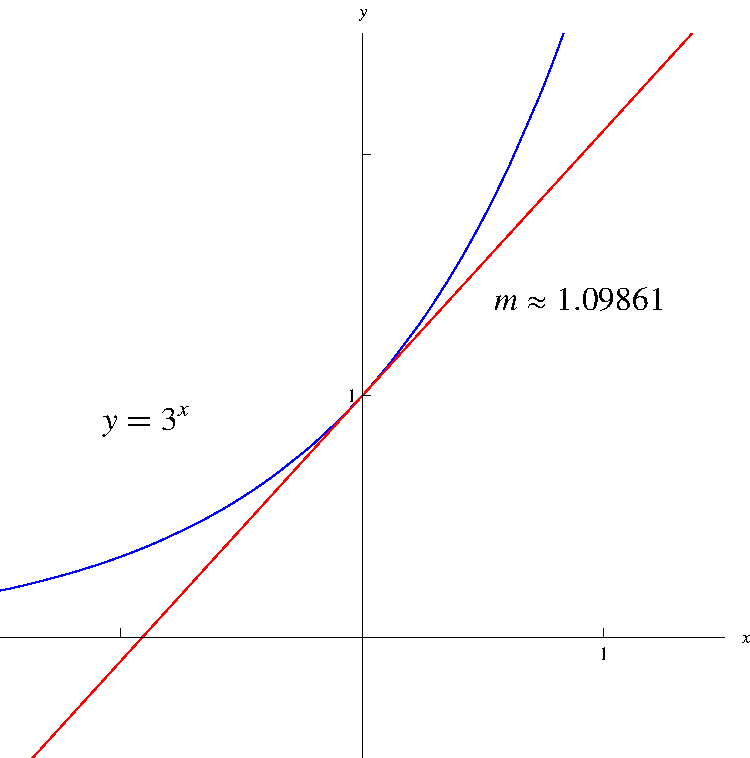
\includegraphics[height=4cm]{exponential-functions/pictures/exp-tangent-three.pdf}%
\end{columns}
\end{frame}
% end module e-def
